% !TeX program = lualatex
% The Deadly Race -- 10-minute talk, local Bitcoin meetup.
% Slides in EN (audience fluent, matches the projected paper); delivery in the vernacular.
% Build:  lualatex deadly-race-10min.tex   (twice, for the frame count)
\documentclass[aspectratio=169,12pt]{beamer}

\usepackage[T1]{fontenc}
\usepackage{lmodern}
\usepackage{tikz}
\usetikzlibrary{arrows.meta,positioning}

\usetheme{default}
\usefonttheme{professionalfonts}
\renewcommand{\familydefault}{\sfdefault}

% --- palette: identical to the manuscript, so the deck and the projected paper match
\definecolor{accent}{HTML}{2F6F4E}
\definecolor{accentdark}{HTML}{234F38}
\definecolor{accentlight}{HTML}{EBF3EE}
\definecolor{darktext}{HTML}{1E1E1E}
\definecolor{graytext}{HTML}{646464}
\definecolor{attackcol}{HTML}{C0392B}
\definecolor{bg}{HTML}{FAFAF7}

% Light background on purpose: survives a weak or badly-aimed projector.
% For a dark room, swap the next two lines' colours (bg <-> darktext) and re-run.
\setbeamercolor{background canvas}{bg=bg}
\setbeamercolor{normal text}{fg=darktext}
\setbeamercolor{frametitle}{fg=accentdark}
\setbeamercolor{structure}{fg=accent}
\setbeamercolor{alerted text}{fg=attackcol}
\setbeamercolor{itemize item}{fg=accent}
\setbeamercolor{itemize subitem}{fg=graytext}

\setbeamertemplate{navigation symbols}{}
\setbeamertemplate{itemize item}{\raisebox{0.15ex}{\tiny$\blacksquare$}}
\setbeamertemplate{itemize subitem}{\raisebox{0.15ex}{\tiny$\square$}}
\setbeamertemplate{frametitle}{%
  \vspace{0.33em}\usebeamerfont{frametitle}\usebeamercolor[fg]{frametitle}%
  \bfseries\insertframetitle\par\vspace{-0.2em}%
  {\color{accent}\rule{\textwidth}{1.1pt}}\par}
\setbeamerfont{frametitle}{size=\Large}
\setbeamertemplate{footline}{%
  \hfill{\color{graytext}\tiny\insertframenumber}\hspace{1.2em}\vspace{0.33em}}

\newcommand{\punch}[1]{{\color{accentdark}\bfseries #1}}
\newcommand{\bad}[1]{{\color{attackcol}\bfseries #1}}

\begin{document}

% ---------------------------------------------------------------- 1. title
{\setbeamertemplate{footline}{}
\begin{frame}[plain]
  \vspace{0.66em}
  {\color{accentdark}\huge\bfseries The Deadly Race\par}
  \vspace{0.28em}
  {\color{darktext}\large When ``graceful recovery'' makes coercion lethal\par}
  \vspace{0.88em}
  {\color{graytext}\rule{0.32\textwidth}{0.8pt}\par}
  \vspace{0.55em}
  {\large Yuri da Silva Villas Boas\par}
  \vspace{0.22em}
  {\color{graytext}\small
   Author, Bitcoin BIP-450 \quad$\cdot$\quad
   % swap to "contributor to" once PR #212 is merged
   contributing to \texttt{jlopp/physical-bitcoin-attacks}\par}
  \vspace{0.77em}
  {\color{graytext}\footnotesize A formal threat model for wrench attacks --- draft, 2026\par}
\end{frame}}

% ---------------------------------------------------------------- 2. it's here
\begin{frame}[t]{Not a foreign problem. Not a historical one.}
  \vspace{0.44em}
  \begin{columns}[T]
    \begin{column}{0.42\textwidth}
      {\color{accentdark}\Huge\bfseries 344\par}
      {\small documented physical-coercion attacks\par
       \color{graytext} Lopp's \texttt{physical-bitcoin-attacks} registry\par}
      \vspace{0.61em}
      {\color{accentdark}\Huge\bfseries 12\par}
      {\small of them in \textbf{Brazil}\par}
    \end{column}
    \begin{column}{0.52\textwidth}
      \vspace{0.22em}
      {\small
      \begin{tabular}{@{}ll@{}}
        \textbf{2024} & 41\\[2pt]
        \textbf{2025} & 85\\[2pt]
        \bad{2026} & \bad{48 so far}\\
      \end{tabular}\par}
      \vspace{0.61em}
      {\footnotesize\color{graytext}
       Brazilian entries include\\
       Florianópolis 2017 $\cdot$ Recife 2021 $\cdot$ São Paulo 2024\\
       Goiânia 2025 $\cdot$ \textbf{Vitória, June 2026} $\cdot$
       \textbf{Ribeirão Preto, July 2026}\par}
    \end{column}
  \end{columns}
  \vfill
  {\small The curve is not flattening, and the victims are not billionaires.}
  \vspace{0.22em}
\end{frame}

% ---------------------------------------------------------------- 3. two failures
\begin{frame}[t]{Our two standard answers do not work here}
  \vspace{0.50em}
  \begin{itemize}\setlength\itemsep{0.77em}
    \item \punch{Cryptography does not help.}\\
      {\small The attacker does not break the cipher. They compel the person who
       operates it. Dolev--Yao, IND-CCA, forward secrecy --- every model we use
       assumes the adversary cannot reach the \emph{holder}.}
    \item \punch{Obscurity is not security.}\\
      {\small ``Never tell anyone you own Bitcoin'' is a bet that the attacker
       does not know something you do. Kerckhoffs settled that in 1883 --- and
       the bet degrades exactly as adoption spreads.}
  \end{itemize}
  \vfill
  {\footnotesize\color{graytext}
   Registry, January 2026, Sweden: a streamer who \emph{had no cryptocurrency
   at all} was invaded and tortured anyway.}
  \vspace{0.22em}
\end{frame}

% ---------------------------------------------------------------- 4. NNPP
\begin{frame}[t]{The thing nobody can do}
  \vspace{0.72em}
  \begin{center}
    {\color{accentdark}\huge\bfseries You cannot prove you forgot.\par}
  \end{center}
  \vspace{0.72em}
  \begin{itemize}\setlength\itemsep{0.49em}
    \item {\small You can hand over a seed. You can open a wallet. You
      \emph{cannot} prove there is no second copy --- in your head, on an SD card,
      steganographic notes in a book, the login to an email account.}
    \item {\small Non-possession is a \textbf{negative existential}. Cooperation only
      ever \emph{raises a lower bound} on what you had; it never certifies the
      upper one.}
    \item \punch{So a rational attacker must assume you kept something} ---
      {\small not from paranoia, but because no evidence could say otherwise.}
  \end{itemize}
  \vspace{0.17em}
  {\footnotesize\color{graytext}Non-Negative-Proof Principle (NNPP)}
\end{frame}

% ---------------------------------------------------------------- 5. the race
\begin{frame}[t]{So the encounter ends --- and the race starts}
  \vspace{0.22em}
  \begin{center}
  \resizebox{\textwidth}{!}{%
  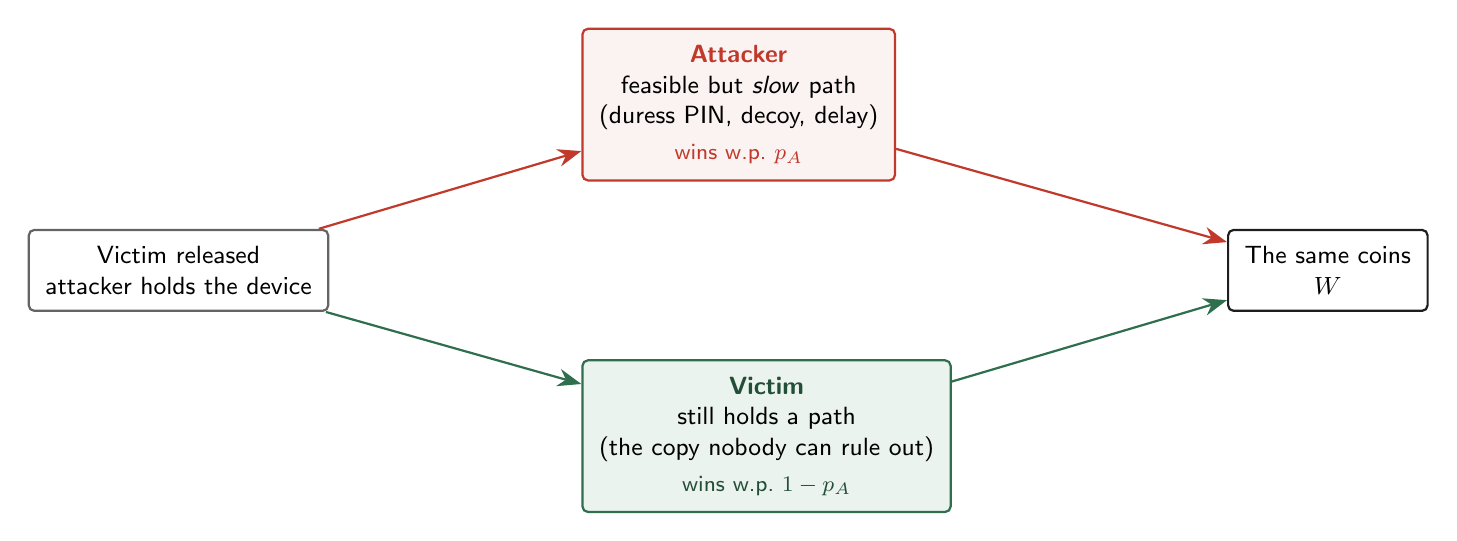
\begin{tikzpicture}[
      >={Stealth[length=3mm]},
      node distance=6mm,
      box/.style={rounded corners=2pt,draw,thick,align=center,inner sep=6pt,font=\small},
      lbl/.style={font=\footnotesize,align=center}]
    \node[box,draw=graytext] (rel) {Victim released\\ attacker holds the device};
    \node[box,draw=attackcol,fill=attackcol!6,above right=6mm and 32mm of rel] (att)
      {\color{attackcol}\textbf{Attacker}\\ feasible but \emph{slow} path\\
       (duress PIN, decoy, delay)\\[2pt]
       {\color{attackcol}\footnotesize wins w.p.\ $p_A$}};
    \node[box,draw=accent,fill=accentlight,below right=6mm and 32mm of rel] (vic)
      {\color{accentdark}\textbf{Victim}\\ still holds a path\\
       (the copy nobody can rule out)\\[2pt]
       {\color{accentdark}\footnotesize wins w.p.\ $1-p_A$}};
    \node[box,draw=darktext,right=32mm of rel,xshift=82mm] (pot)
      {The same coins\\ \textbf{$W$}};
    \draw[->,thick,attackcol] (rel) -- (att);
    \draw[->,thick,accent]    (rel) -- (vic);
    \draw[->,thick,attackcol] (att) -- (pot);
    \draw[->,thick,accent]    (vic) -- (pot);
  \end{tikzpicture}}
  \end{center}
  {\small Both parties can still reach the funds. That is a \punch{gray outcome}:
   $0 < p_A < 1$.}
\end{frame}

% ---------------------------------------------------------------- 6. the lemma
\begin{frame}[t]{What the second racer is worth --- dead}
  \vspace{0.61em}
  \begin{center}
    {\small Expected take with the victim alive and racing:}\\[0.2em]
    {\Large $p_A\,W$}\\[0.6em]
    {\small Expected take with the victim removed:}\\[0.2em]
    {\Large $W$}\\[0.7em]
    {\color{accentdark}\rule{0.5\textwidth}{0.8pt}}\\[0.6em]
    {\color{attackcol}\huge\bfseries $(1-p_A)\,W > c$}\\[0.5em]
    {\small The attacker acts on the difference when it beats the cost $c$.}
  \end{center}
  \vfill
  {\footnotesize\color{graytext}
   And by NNPP, \emph{the only instrument available} for pushing $p_A$ toward 1
   is removing the other racer --- no promise, no surrender, no cooperation can
   substitute for it.}
  \vspace{0.17em}
\end{frame}

% ---------------------------------------------------------------- 7. punchline
\begin{frame}[t]{Now read the inequality backwards}
  \vspace{0.4em}
  \begin{center}
    {\large The \emph{gentler} the fallback, the \emph{smaller} $p_A$.\par}
    \vspace{0.28em}
    {\large The smaller $p_A$, the \bad{larger $(1-p_A)\,W$}.\par}
    \vspace{0.6em}
    {\color{accentdark}\Large\bfseries
     Graceful degradation --- a virtue everywhere else in engineering ---\\[0.2em]
     is here a \bad{murder incentive}.\par}
  \end{center}
  \vfill
  {\small A scheme that simply hands the attacker everything kills nobody.
   \punch{The graceful fallback is worse than that.}}\\[0.35em]
  {\footnotesize\color{graytext}
   The designs that market themselves as the safest sit squarely in the region of
   maximum assassination incentive.}
\end{frame}

% ---------------------------------------------------------------- 8. the bar
\begin{frame}[t]{The bar: No Gray Area}
  \vspace{0.35em}
  \begin{center}
  \resizebox{\textwidth}{!}{%
  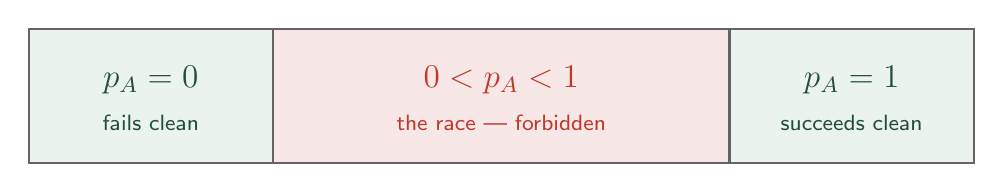
\begin{tikzpicture}[font=\small]
    \fill[accentlight] (0,0) rectangle (3.1,1.7);
    \fill[attackcol!12] (3.1,0) rectangle (8.9,1.7);
    \fill[accentlight] (8.9,0) rectangle (12,1.7);
    \draw[thick,graytext] (0,0) rectangle (12,1.7);
    \draw[thick,graytext] (3.1,0) -- (3.1,1.7);
    \draw[thick,graytext] (8.9,0) -- (8.9,1.7);
    \node at (1.55,1.05) {\color{accentdark}\large\bfseries $p_A = 0$};
    \node at (1.55,0.5) {\color{accentdark}\footnotesize fails clean};
    \node at (6.0,1.05) {\color{attackcol}\large\bfseries $0 < p_A < 1$};
    \node at (6.0,0.5) {\color{attackcol}\footnotesize the race --- forbidden};
    \node at (10.45,1.05) {\color{accentdark}\large\bfseries $p_A = 1$};
    \node at (10.45,0.5) {\color{accentdark}\footnotesize succeeds clean};
  \end{tikzpicture}}
  \end{center}
  \vspace{0.61em}
  \begin{itemize}\setlength\itemsep{0.39em}
    \item {\small Every encounter must resolve to a \textbf{clear} endpoint.
      \punch{Either you lose clean, or you win clean. Never a race.}}
    \item {\small The two endpoints are not equally \emph{pleasant} --- $p_A=1$
      costs you the funds --- but both are \textbf{survivable}.}
    \item {\small Coercion resistance is a bar on \punch{the holder's safety} first,
      and only then on the funds.}
  \end{itemize}
\end{frame}

% ---------------------------------------------------------------- 9. R1/R2
\begin{frame}[t]{Exactly two ways to clear it}
  \vspace{0.39em}
  \begin{columns}[T]
    \begin{column}{0.47\textwidth}
      {\color{accentdark}\large\bfseries (R1) Remove the race\par}
      \vspace{0.22em}
      {\small No feasible seizure path exists at all $\Rightarrow p_A = 0$.\par}
      \vspace{0.33em}
      {\small Custody stays \textbf{individual}.\par}
      \vspace{0.33em}
      {\footnotesize\color{graytext} The harder road. This is what my construction
       attempts --- and it is \emph{research}, not a product.\par}
    \end{column}
    \begin{column}{0.47\textwidth}
      {\color{accentdark}\large\bfseries (R2) Winner out of reach\par}
      \vspace{0.22em}
      {\small The party who \emph{will} win is a remote delegate the attacker
       cannot touch.\par}
      \vspace{0.33em}
      {\small Custody becomes \textbf{shared} --- you pay with a trusted party.\par}
      \vspace{0.33em}
      {\footnotesize\color{graytext} Timelock-rescue vaults with a remote
       co-signer. \textbf{This ships today.}\par}
    \end{column}
  \end{columns}
  \vfill
  {\small If you take one practical thing from tonight: \punch{R2 is the option
   that already exists.}}
  \vspace{0.22em}
\end{frame}

% ---------------------------------------------------------------- 10. close
\begin{frame}[t]{The crypto isn't broken. The incentive is.}
  \vspace{0.55em}
  {\small And it lives in a layer our threat models leave out.\par}
  \vspace{0.66em}
  \begin{itemize}\setlength\itemsep{0.35em}
    \item {\small Paper (draft): \texttt{github.com/Yuri-SVB/great-wall-docs}\\
      \hspace*{1.2em}\texttt{papers/wrench-attack-threat-model}}
    \item {\small Registry: \texttt{github.com/jlopp/physical-bitcoin-attacks}}
    \item {\small BIP-450 $\cdot$ \texttt{github.com/Yuri-SVB}}
  \end{itemize}
  \vspace{0.66em}
  {\color{accentdark}\large\bfseries
   It is a draft, and I would rather it be attacked than admired.\par}
  \vspace{0.50em}
  {\small Come find me if you want to (a) poke holes in it, (b) tell me about a
   Brazilian case that is not in the registry --- I contribute to it, and I will
   add it --- or (c) just get the link.}
\end{frame}

% ================================================================ backup
\appendix

{\setbeamertemplate{footline}{}
\begin{frame}[plain]
  \vspace{1.76em}
  \begin{center}{\color{graytext}\Large Backup slides --- Q\&A}\end{center}
\end{frame}}

\begin{frame}[t]{``Doesn't multisig solve this?''}
  \vspace{0.55em}
  \begin{itemize}\setlength\itemsep{0.56em}
    \item {\small Only if it clears the bar. \punch{Reachable co-signers who can be
      coerced one at a time is a race with extra steps.}}
    \item {\small R2 works \textbf{only} when the deciding party is genuinely
      beyond the attacker's reach.}
    \item {\small Honest cost of R2: its safety rests on the delegate
      \emph{refusing a legitimate owner pleading for their life}. The refusal that
      defeats the coerced plea also defeats the genuine one.}
    \item {\small And an access-dominating delegate is \punch{not self-custody} ---
      it reinstates the counterparty the design set out to remove.}
  \end{itemize}
\end{frame}

\begin{frame}[t]{``Real attackers aren't rational calculators.''}
  \vspace{0.66em}
  \begin{itemize}\setlength\itemsep{0.63em}
    \item {\small The model is deliberately \punch{\emph{a fortiori}}: it endows the
      attacker with the \emph{most kill-prone} reasoning available and asks whether
      the design survives anyway.}
    \item {\small It is a \textbf{floor}, not a claim that every attacker computes an
      expected value.}
    \item {\small Same move for Kerckhoffs and for NNPP: give the adversary
      everything, then demand safety.}
  \end{itemize}
  \vfill
  {\footnotesize\color{graytext}
   ``If, even after maximizing the attacker's proclivity to enact the deadly race,
   killing still buys it nothing, the method is deadly-race-safe.''}
  \vspace{0.17em}
\end{frame}

\begin{frame}[t]{The open question I have not closed}
  \vspace{0.55em}
  {\small The R1 route needs a secret that \textbf{cannot be transmitted} --- one you
   can use but cannot hand over. That means tacit, perceptual recall
   (\emph{TKBA}), not a memorised string.\par}
  \vspace{0.55em}
  \begin{itemize}\setlength\itemsep{0.42em}
    \item {\small It is the \punch{load-bearing assumption} of the construction.}
    \item {\small It cannot be settled by argument --- it needs \textbf{measurement}:
      how reliably do people re-point a memorised location, over realistic
      intervals, against an explicit false-reject target?}
    \item {\small Spaced repetition addresses \emph{maintenance} of recall, not the
      base rate.}
  \end{itemize}
  \vspace{0.44em}
  {\small That is an open question, not a hole I have papered over --- and it is the
   sharpest critique the work has drawn so far.}
\end{frame}

\begin{frame}[t]{``Isn't publishing this irresponsible?''}
  \vspace{0.61em}
  \begin{itemize}\setlength\itemsep{0.56em}
    \item {\small The incentive is \punch{disclosed, not created}. It is already a
      property of the situation a coercer faces.}
    \item {\small Kerckhoffs again: assume they understand the landscape. Not
      publishing is a bet on obscurity --- and the registry is the record of that
      bet losing.}
    \item {\small Publishing the danger \emph{together with a bar that rejects the
      designs causing it} is net-protective.}
    \item {\small \punch{Coldcard's five quiet years were not obscurity working ---
      they were the exposed population compounding.} Delay never chooses between
      attack and no attack, only between a smaller reckoning now and a larger one
      later.}
  \end{itemize}
  \vfill
  {\footnotesize\color{graytext}
   Not peer reviewed. First manuscript, 2026, in preparation --- said plainly.}
  \vspace{0.17em}
\end{frame}

\end{document}
